\chapter{List Views}
\label{LV}

\section{Introduction}
\label{LV:introduction}
\texttt{ListView} is actually a \textit{view group} that contains a list of scrollable items. (Roughly you can think of a list view as a vertical linear layout combined with a scroll bar and a bunch of other functionality!). Just like a vertical linear layout, in a list view you can put simple text view OR very complex layouts inside each row:

\begin{center}
	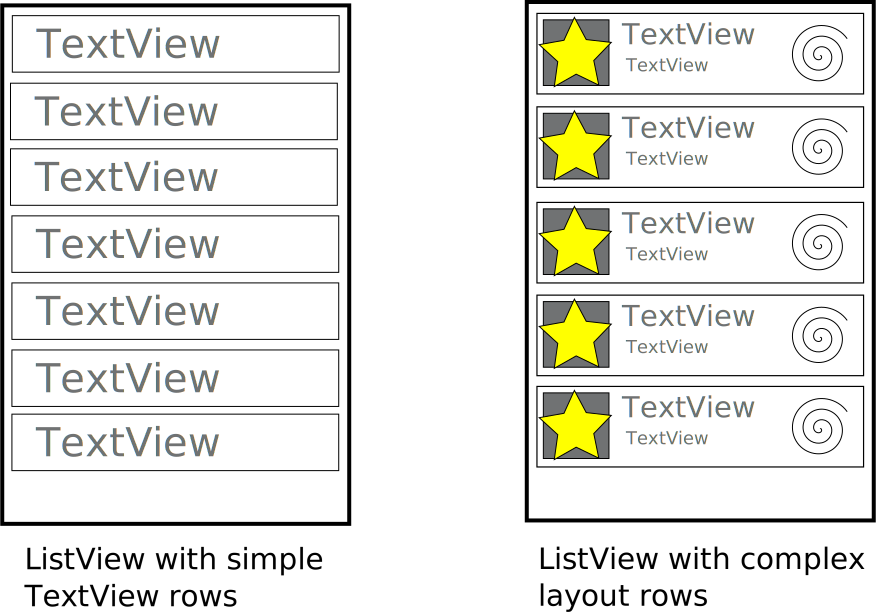
\includegraphics[scale=0.35]{chapters/ch10/images/1}
\end{center}

\begin{quote}
	\textit{``By default each row of the list view contains a single \texttt{TextView} element''.}
\end{quote}

\section{Create New Project}
\label{LV:createProj}

Create a new project from scratch. Perform the following steps:
\begin{enumerate}
	\item Create a new project having name ``\texttt{Chapter\ref{LV}}''
	\item Select minimum API 16 : Android 4.1 (Jelly Bean).
	\item Select ``\texttt{Empty Activity}''
	\item Accept default values for activity and click finish. \\
\end{enumerate}

\section{Populating ListView}
\subsection{Through XML}
Open up to \texttt{activity\_main.xml} and switch to text mode to view its XML code. Change the root layout to \texttt{LinearLayout}. Delete some of its attributes such as padding. Add the orientation attribute and set it to ``vertical'' (line 8). Also remove the default \texttt{TextView} to match the following:

\begin{center}
	\includegraphics[scale=0.4]{chapters/ch10/images/2}
\end{center}

Now change to design mode and drag a ``\textit{list view}'' (from the Containers group) on top of the linear layout. Set list view's width to ``\texttt{match\_parent}'' and it's height to ``\texttt{wrap\_content}'' :

\begin{center}
	\includegraphics[scale=0.4]{chapters/ch10/images/3}
\end{center}

Open ``\texttt{strings.xml}'' and add an ``\texttt{string-array}'' element. This is basically an array of strings. Give it a name such as ``\texttt{employee\_names}'' Each string in this array is specified using an ``\texttt{item}'' tag (lines 4 to 13):

\begin{center}
	\includegraphics[scale=0.4]{chapters/ch10/images/4}
\end{center}

Now open ``\texttt{activity\_main.xml}'' and switch to the text mode. Inside the \texttt{ListView} element add an attribute called ``\texttt{android:entries}'' and assign it a value of ``\texttt{@array/employee\_names}'': (line 14 below):

\begin{center}
	\includegraphics[scale=0.4]{chapters/ch10/images/5}
\end{center}

Switch to the design mode and you will see list view updated with employee names. Also run the app on a device to see the list view in action. Right now clicking on any cell won't do anything but we will soon fix this. \\

The benefit of adding data through XML is that it is easier than other approaches. The drawback, big one, is that the data is fixed and hard coded. Once created you can't grow or shrink the array at runtime.

\subsubsection{Exercise}
Add about 10 more employees to the string array and run the app on a device. Can you scroll the list?

\subsection{Through Java Code}
Before we can proceed, we have to understand the concept of an ``Array Adapter''. 

\subsubsection{The Array Adapter}
The array adapter acts as a glue between the data source and the list view:

\begin{center}
	\includegraphics[scale=0.4]{chapters/ch10/images/6}
\end{center}

For each row in the data source the array adapter creates or ``inflates'' a \texttt{View} for the corresponding row in the list view. In a sense list view is nothing more than an empty shell that is being fed view objects by the array adapter. 

\begin{quote}
	\textit{``By default the array adapter assumes an array of strings as a data source and spits out rows containing a single \texttt{TextView} for the list view. We need to extend the \texttt{ArrayAdapter} class if we want to work with complex data other than strings or if we want to show complex layouts inside list view rows''}.
\end{quote}

Continuing from the previous section open up \texttt{activity\_main.xml} and switch to text mode. Delete the ``\texttt{android:entries}'' tag (line 14 that we added above). Assign an id ``\texttt{employeeList}'' to the list view. The list view element should look like following:

\begin{center}
	\includegraphics[scale=0.4]{chapters/ch10/images/7}
\end{center}

Open up \texttt{MainActivity.java} and in \texttt{onCreate} function, add an array of strings which will act as the data source. Also obtain the reference to our \texttt{ListView} that we added initially (lines 14-21):

\begin{center}
	\includegraphics[scale=0.4]{chapters/ch10/images/8}
\end{center}

Final step is to create an \texttt{ArrayAdapter} object and attach it to the list view. Add the following code right after line 21:

\begin{center}
	\includegraphics[scale=0.4]{chapters/ch10/images/9}
\end{center}

Let's review the code line by line:

\begin{itemize}
	\item \textit{Line 22:} The array adapter constructor that we're using accepts three arguments. First one is the current context which will be '\texttt{this}' in most cases.
	
	\item \textit{Line 23:} Here you specify the layout that will be used to create each list view row. We are using a default layout provided by android named \texttt{simple\_list\_item\_1}. This is why we added the \texttt{android} keyword before the name because it belongs to the android namespace.
	
	\item \textit{Line 24:} Specify the data source, which in this case, is an array of strings that we created earlier.
	
	\item \textit{Line 25:}  Finally attach the array adapter object to the list view.
\end{itemize}

Run this app and you will see a bunch of entries in the list view. As usual you can click these but nothing will happen yet. \\

Let's explore \texttt{simple\_list\_item\_1} a bit more. Go to line 23 and right click on the \texttt{simple\_list\_item\_1} name, a popup menu will appear. Select ``Go to $\rightarrow Declaration$'', an xml file named \texttt{simple\_list\_item\_1.xml} will open up in the designer window. If you look at it closely you'll notice that this layout file contains only one \texttt{TextView} widget, exactly as we claimed earlier:

\begin{center}
	\includegraphics[scale=0.4]{chapters/ch10/images/10}
\end{center}

You can also switch to text mode and take a look at its xml source code.

\subsection{Providing Complex Data Source}

